%%%%%%%%%%%%%%%%%%%%%%%%%%%%%%%%%%%%%%%%%
% baposter Landscape Poster
% LaTeX Template
% Version 1.0 (11/06/13)
%
% baposter Class Created by:
% Brian Amberg (baposter@brian-amberg.de)
%
% This template has been downloaded from:
% http://www.LaTeXTemplates.com
%
% License:
% CC BY-NC-SA 3.0 (http://creativecommons.org/licenses/by-nc-sa/3.0/)
%
%%%%%%%%%%%%%%%%%%%%%%%%%%%%%%%%%%%%%%%%%

%----------------------------------------------------------------------------------------
%	PACKAGES AND OTHER DOCUMENT CONFIGURATIONS
%----------------------------------------------------------------------------------------


\documentclass[landscape,a0paper,fontscale=0.36]{baposter} % Adjust the font scale/size here (was 0.285)


\usepackage{graphicx} % Required for including images

\usepackage{amsmath} % For typesetting math
\usepackage{amssymb} % Adds new symbols to be used in math mode
\usepackage{upgreek}
\usepackage{bm}

\usepackage{booktabs} % Top and bottom rules for tables
\usepackage{enumitem} % Used to reduce itemize/enumerate spacing
\usepackage{palatino} % Use the Palatino font
\usepackage[font=small,labelfont=bf]{caption} % Required for specifying captions to tables and figures

\usepackage{multicol} % Required for multiple columns
\setlength{\columnsep}{1.5em} % Slightly increase the space between columns
\setlength{\columnseprule}{0mm} % No horizontal rule between columns

\usepackage{tikz} % Required for flow chart
\usetikzlibrary{shapes,arrows} % Tikz libraries required for the flow chart in the template

\newcommand{\compresslist}{ % Define a command to reduce spacing within itemize/enumerate environments, this is used right after \begin{itemize} or \begin{enumerate}
\setlength{\itemsep}{1pt}
\setlength{\parskip}{0pt}
\setlength{\parsep}{0pt}
}

\usepackage[superscript,biblabel]{cite}

\definecolor{lightblue}{rgb}{0.145,0.6666,1} % Defines the color used for content box headers
\definecolor{ucmaroon}{cmyk}{0, 1, 0.7, 0.5}
\definecolor{ucdarkgray}{cmyk}{0, 0.05, 0.1, 0.6}
\definecolor{uclightgray}{cmyk}{0, 0, 0.05, 0.2}

\begin{document}

\background{
  \begin{tikzpicture}[remember picture,overlay]
    \fill[fill=uclightgray] (current page.north west) rectangle (current page.south east); %the poster background color
    \fill [fill=ucmaroon] (current page.north west) rectangle ([yshift=-\headerheight] current page.north east);     %the header
  \end{tikzpicture}
}

\begin{poster}
{
headerborder=closed, % Adds a border around the header of content boxes
colspacing=1em, % Column spacing
background=user,
% bgColorOne=uclightgray, % Background color for the gradient on the left side of the poster
% bgColorTwo=uclightgray, % Background color for the gradient on the right side of the poster
borderColor=black, % Border color
headerColorOne=ucmaroon, % Background color for the header in the content boxes (left side)
headerColorTwo=ucmaroon, % Background color for the header in the content boxes (right side)
headerFontColor=white, % Text color for the header text in the content boxes
boxColorOne=white, % Background color of the content boxes
textborder=roundedleft, % Format of the border around content boxes, can be: none, bars, coils, triangles, rectangle, rounded, roundedsmall, roundedright or faded
eyecatcher=false, % Set to false for ignoring the left logo in the title and move the title left
headerheight=0.17\textheight, % Height of the header
headershape=roundedright, % Specify the rounded corner in the content box headers, can be: rectangle, small-rounded, roundedright, roundedleft or rounded
headerfont=\Large\bf\textsc, % Large, bold and sans serif font in the headers of content boxes
%textfont={\setlength{\parindent}{1.5em}}, % Uncomment for paragraph indentation
linewidth=2pt % Width of the border lines around content boxes
}
%----------------------------------------------------------------------------------------
%	TITLE SECTION 
%----------------------------------------------------------------------------------------
%
{
\includegraphics[height=0.5\headerheight]{figs/seal_white.eps}} % First university/lab logo on the left
{\color{white}\Huge{\bf Towards whole-brain validation of diffusion MRI \\[6pt]fiber-orientation distributions with x-ray microcomputed tomography}\vspace{0.75em}} % Poster title
{\color{white}\LARGE{\underline{Scott Trinkle}$^{1}$, \ Sean Foxley$^{1}$, \ Narayanan Kasthuri$^{2}$, \ Patrick La Rivi\`ere$^{1}$} \vspace{0.35em}\\
  \normalsize{$^{1}$Department of Radiology, University of Chicago, \ $^{2}$Department of Neurobiology, University of Chicago}} % Author names and institution
{
\includegraphics[height=0.45\headerheight]{figs/logos/logo_white.eps}} % Second university/lab logo on the right

%----------------------------------------------------------------------------------------
%	Introduction
%----------------------------------------------------------------------------------------

\headerbox{Background and Purpose}{name=intro,column=0,row=0}{
  \vspace{0.5em}
  
    Diffusion MRI (dMRI) is a powerful, non-invasive tool for characterizing
    three-dimensional (3D) tissue microstructure on a macroscopic scale.\newline

    New methods of reconstructing 3D fiber orientation distributions (FODs)
    from dMRI data are rapidly being developed.\newline

    Previous efforts to validate these FODs have relied on ground truth
    histological data with non-isotropic resolution over small regions of
    interest (ROI).\cite{Schilling2018}

  \vspace{0.5em}

  \begin{center}
      \large{\textbf{In this study, we demonstrate a pipeline for \newline the use of natively isotropic,
  synchrotron \newline x-ray microcomputed tomography ($\bm{\upmu}$CT) data to \newline validate dMRI FODs
  over a whole mouse brain.}}
  \end{center}

\vspace{0.3em} % When there are two boxes, some whitespace may need to be added if the one on the right has more content
}

%----------------------------------------------------------------------------------------
%	$\upmu$CT FODs
%----------------------------------------------------------------------------------------

\headerbox{$\upmu$CT FOD Construction}{name=xrayfods,column=0,row=0,above=bottom, below=intro}{
  \vspace{0.5em}
  
  For a 3D intensity image $f(x,y,z)$, the fiber orientation at each voxel is
  given by the eigenvector corresponding to the smallest eigenvalue of the
  structure tensor:
  
  \begin{align}
    \text{ST}\left(f\right) &= g_{\sigma_N} \circledast
    \begin{pmatrix}
      f_x^2 & f_x f_y & f_x f_z \\
      f_x f_y & f_y^2 & f_y f_z \\
      f_x f_z & f_y f_z & f_z^2 \\
    \end{pmatrix}
    \nonumber
  \end{align}

  \begin{center}
    \begin{tabular}{r l}
      $\circledast$ : &convolution\\[6pt]
      $g_{\sigma}$ : &Gaussian with standard deviation $\sigma$\\[6pt]
      $f_x, f_y, f_z$ : &partial derivative images of $f$
    \end{tabular}
  \end{center}

  \vspace{1.5em}

  In an ROI containing $K$ such fiber orientation vectors, the FOD can be written in spherical coordinates:
  
  \begin{align}
    \text{FOD}(\theta, \phi) = \frac{1}{K}\sum_{k=1}^K \delta(\theta - \theta_k)\delta(\phi - \phi_k)\nonumber
  \end{align}

  The FOD can be expanded on the real spherical harmonics, $Y_l^m$, up to degree $L_{max}$\cite{Alimi2018}:

  \begin{align}
    \hat{\text{FOD}}(\theta, \phi) &= \sum_{l=0}^{L_{max}}\sum_{m=-l}^l c_{lm}Y_l^m(\theta, \phi)\nonumber\\[6pt]
    c_{lm} &= \frac{1}{K}\sum_{k=1}^K Y_l^m(\theta_k, \phi_k)\nonumber
  \end{align}
}


%----------------------------------------------------------------------------------------
%	Data Acquisition
%----------------------------------------------------------------------------------------

\headerbox{Data Acquisition}{name=data,column=1,span=2,row=0}{
\vspace{1em}
\tikzstyle{block} = [rectangle, draw, fill=uclightgray, text centered, rounded corners, minimum height=3em, minimum width=10em]
\begin{center}
\begin{tikzpicture}[scale=0.60]
    \node [block] (mriprep) at (0,0){
      \begin{tabular}{c}
        \textbf{Perfusion-fixed}\\
        \textbf{mouse brain}
      \end{tabular}
    };
    \node [block] (dmriacq) at (8, 0){\textbf{dMRI Acquisition}};
    \draw[->, double] (mriprep) to (dmriacq);
    \node (mrispecs) at (8, -3){
      \small{\begin{tabular}{c}
          Bruker 9.4 T Magnet\\
          150 $\upmu$m isotropic resolution\\
          b-value: 3000 s/mm$^2$\\
          30 uniformly distributed directions
        \end{tabular}}        
    };
    \draw[-, double] (dmriacq) to (mrispecs);
    \node [block] (mrifods) at (8, -7){\textbf{dMRI FODs}};
    \draw[->, double] (mrispecs) to (mrifods);
    \node [block] (xrayprep) at (16,0){\textbf{Sample staining}};
    \draw[->, double] (dmriacq) to (xrayprep);
    \node (stainnotes) at (16, -2.75){
      \small{\begin{tabular}{c}
               uranyl acetate\\
               osmium tetroxide\\
               lead citrate\\
        \end{tabular}}
    };
    \draw[-, double] (xrayprep) to (stainnotes);
    \node [block] (xrayacq) at (24, 0){\textbf{$\bm{\upmu}$CT Acquisition}};
    \draw[->, double] (xrayprep) to (xrayacq);
  \node (xrayspecs) at (24, -2.75){
    \small{\begin{tabular}{c}
        APS at Argonne National Lab\\
        Mosaic sinogram stitching \cite{Vescovi2017}\\
        2.4 $\upmu$m isotropic resolution\\
      \end{tabular}}
  };
  \draw[-, double] (xrayacq) to (xrayspecs);
  \node [block] (xrayfods) at (24, -7){\textbf{$\bm{\upmu}$CT FODs}};
  \draw[->, double] (xrayspecs) to (xrayfods);
  \draw[<->, dashed] (mrifods) to (xrayfods);
  \node (compare) at (16, -7.5) {\small{Quantitative comparison}};
\end{tikzpicture}
\end{center}
\vspace{0.5em}
}


%----------------------------------------------------------------------------------------
%	RESULTS
%----------------------------------------------------------------------------------------

\headerbox{Results}{name=results, column=1, span=2, below=data, above=bottom}{
  \vspace{1em}
  \setlength{\columnsep}{1.0em}

  \begin{multicols}{2}

    \begin{center}
      \includegraphics[width=\linewidth]{figs/real_data/sl3340}\\[3pt]
      \begin{tabular}{c c}
        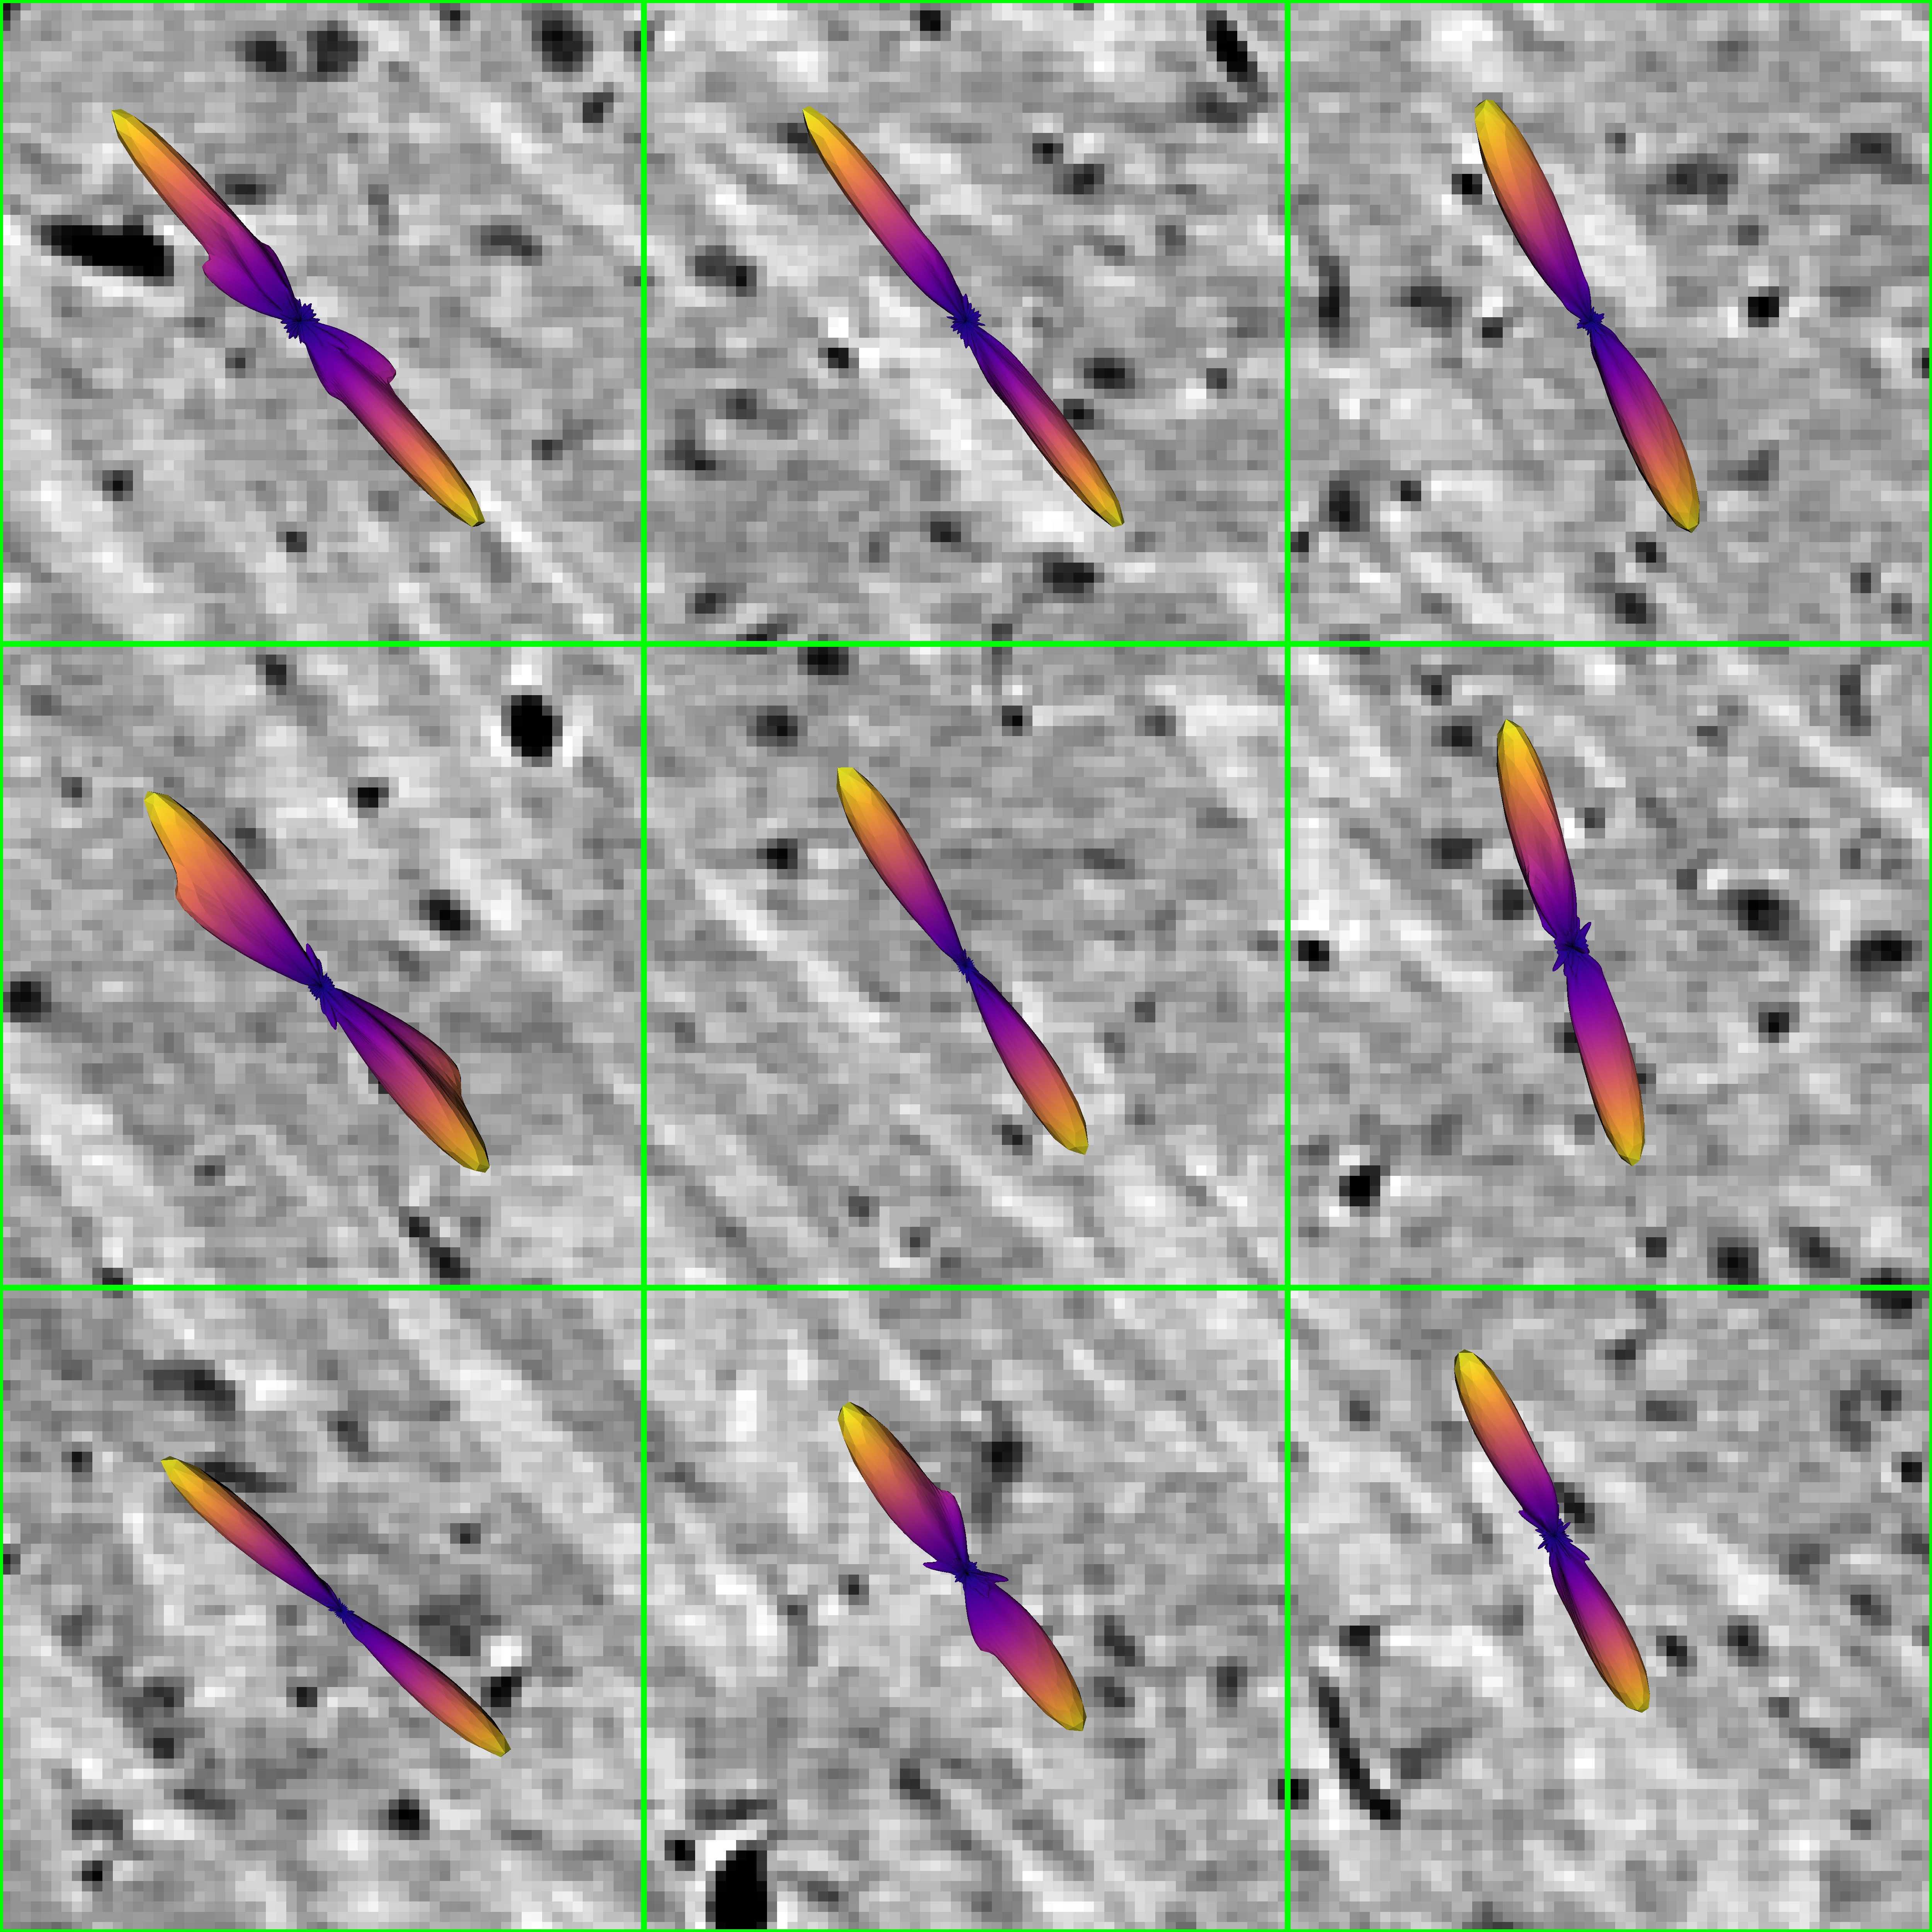
\includegraphics[width=0.4\linewidth]{figs/real_data/UK1} & 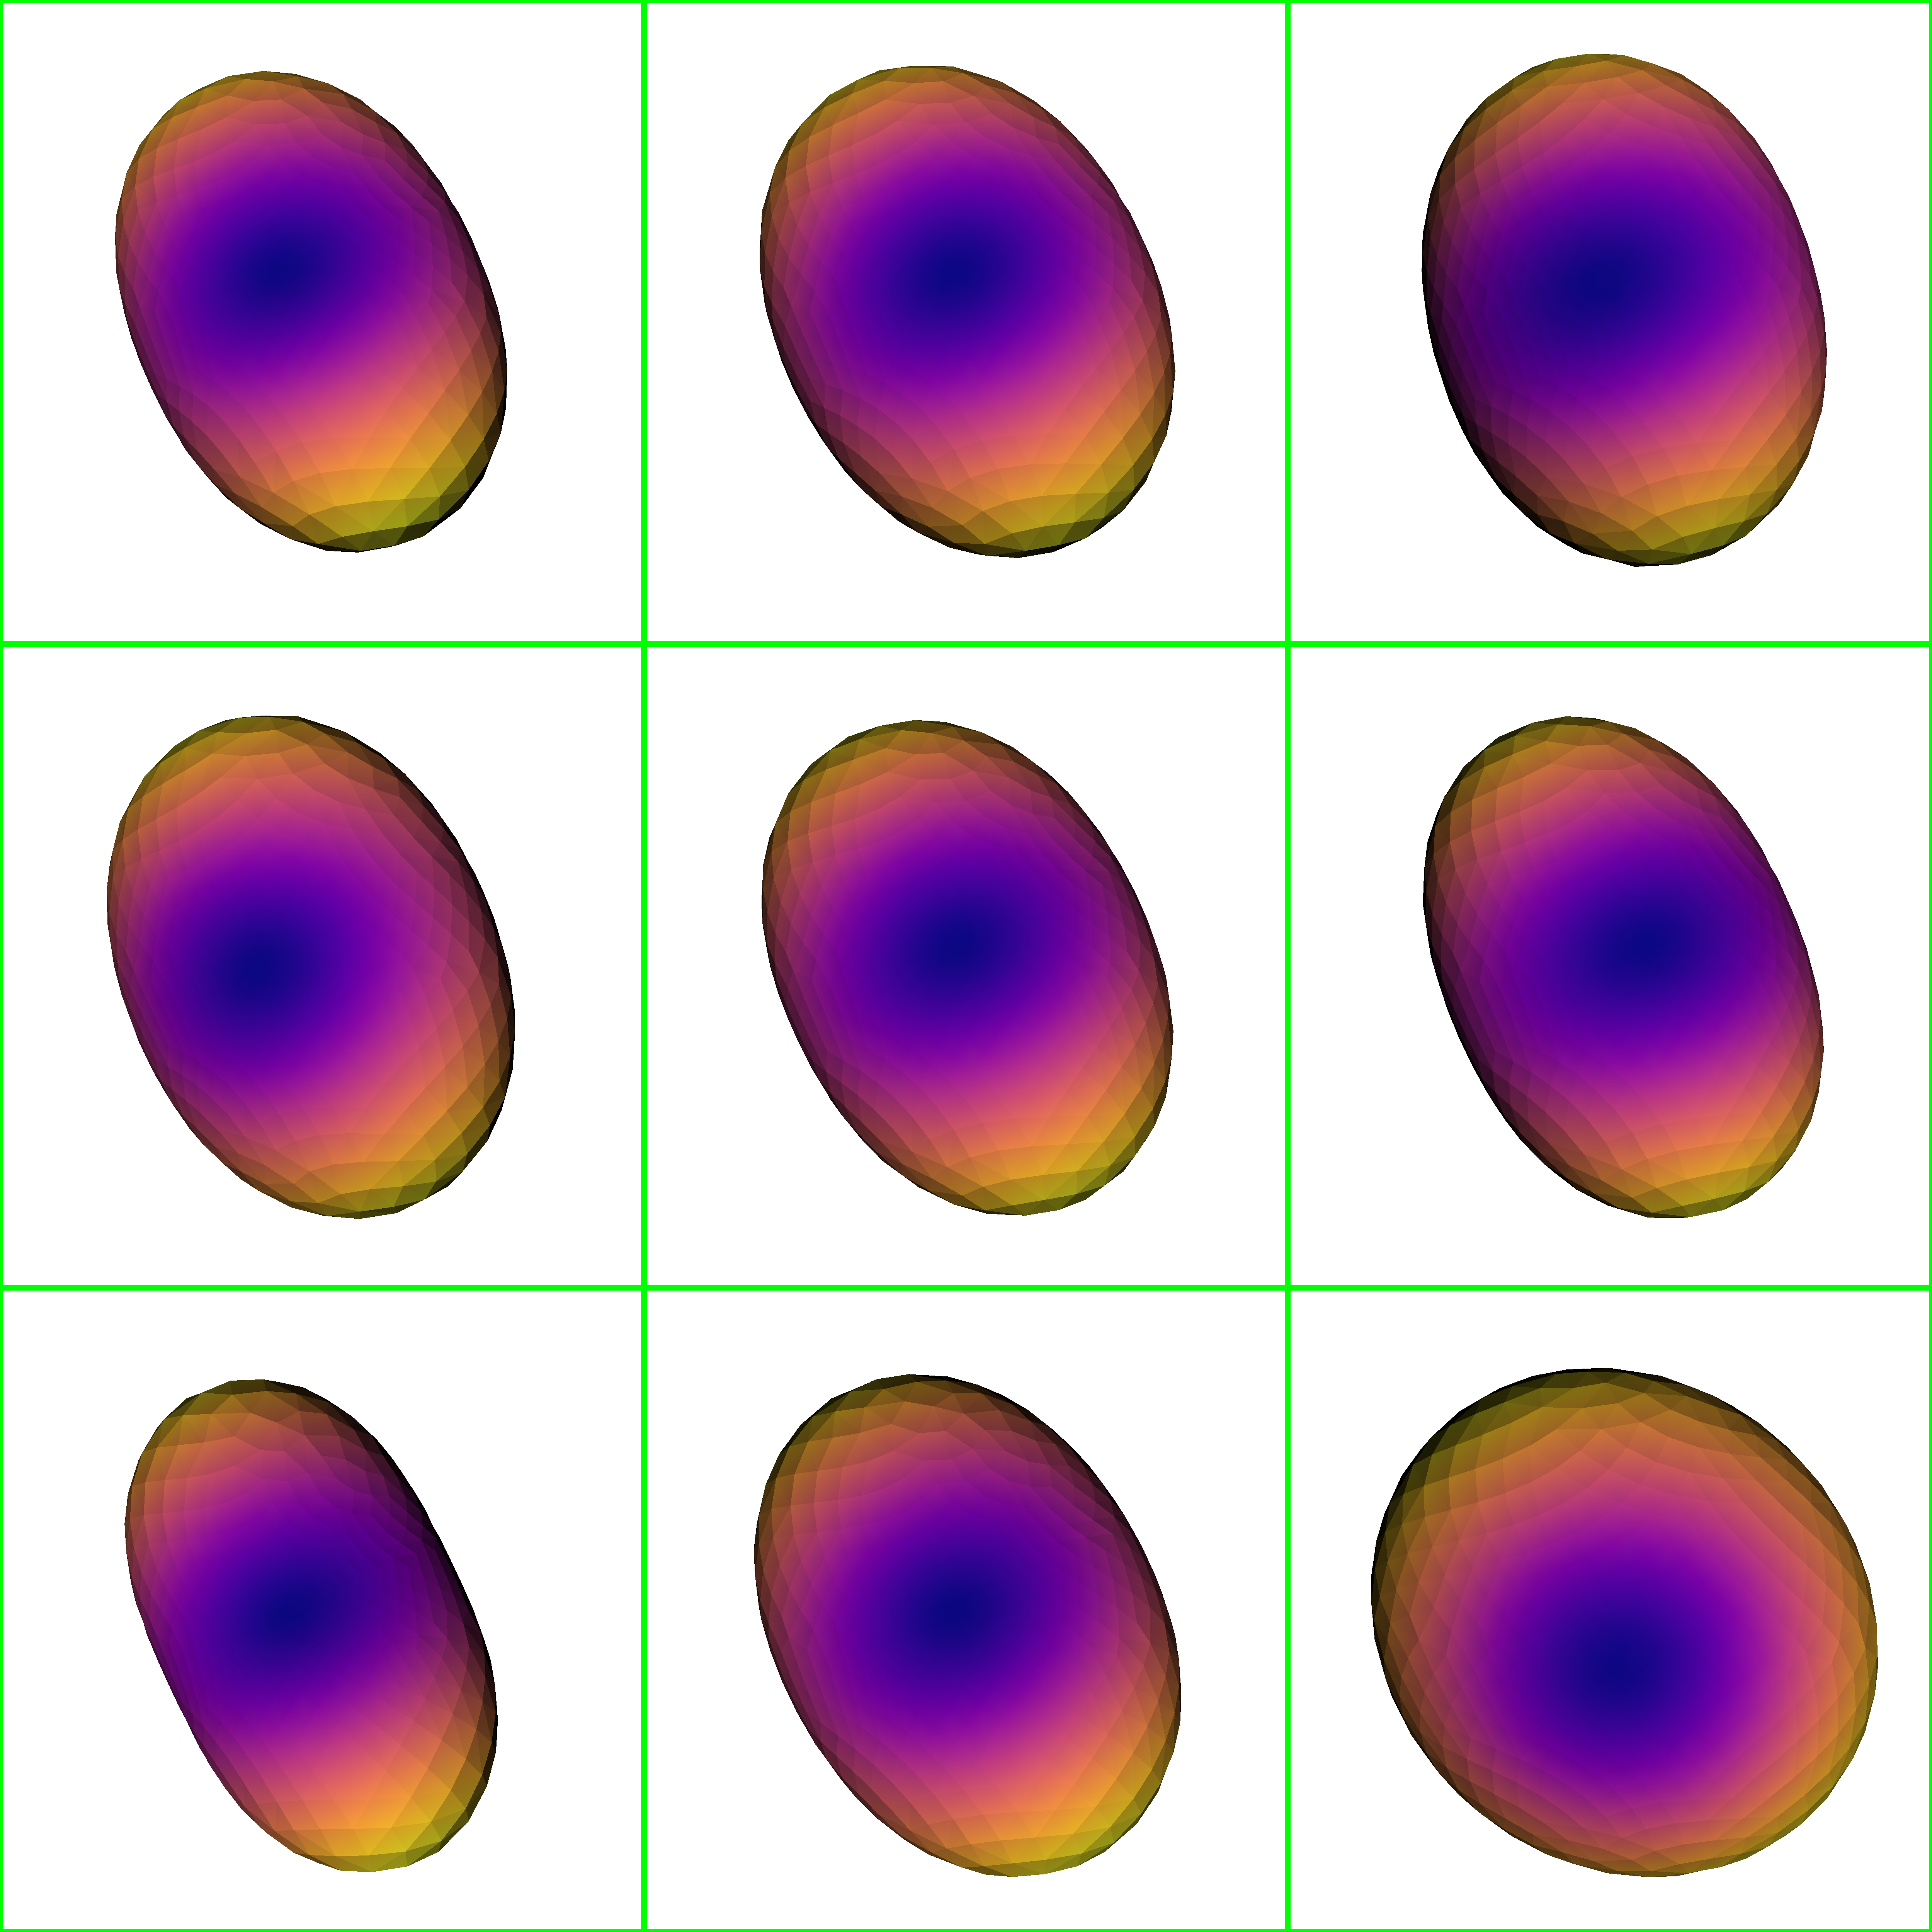
\includegraphics[width=0.4\linewidth]{figs/real_data/UK1_DTI}\\
        $\upmu$CT FODs & DTI FODs
      \end{tabular}
    \end{center}
    
    \begin{center}
      \includegraphics[width=\linewidth]{figs/real_data/sl4530}\\[3pt]
      \begin{tabular}{c c}
        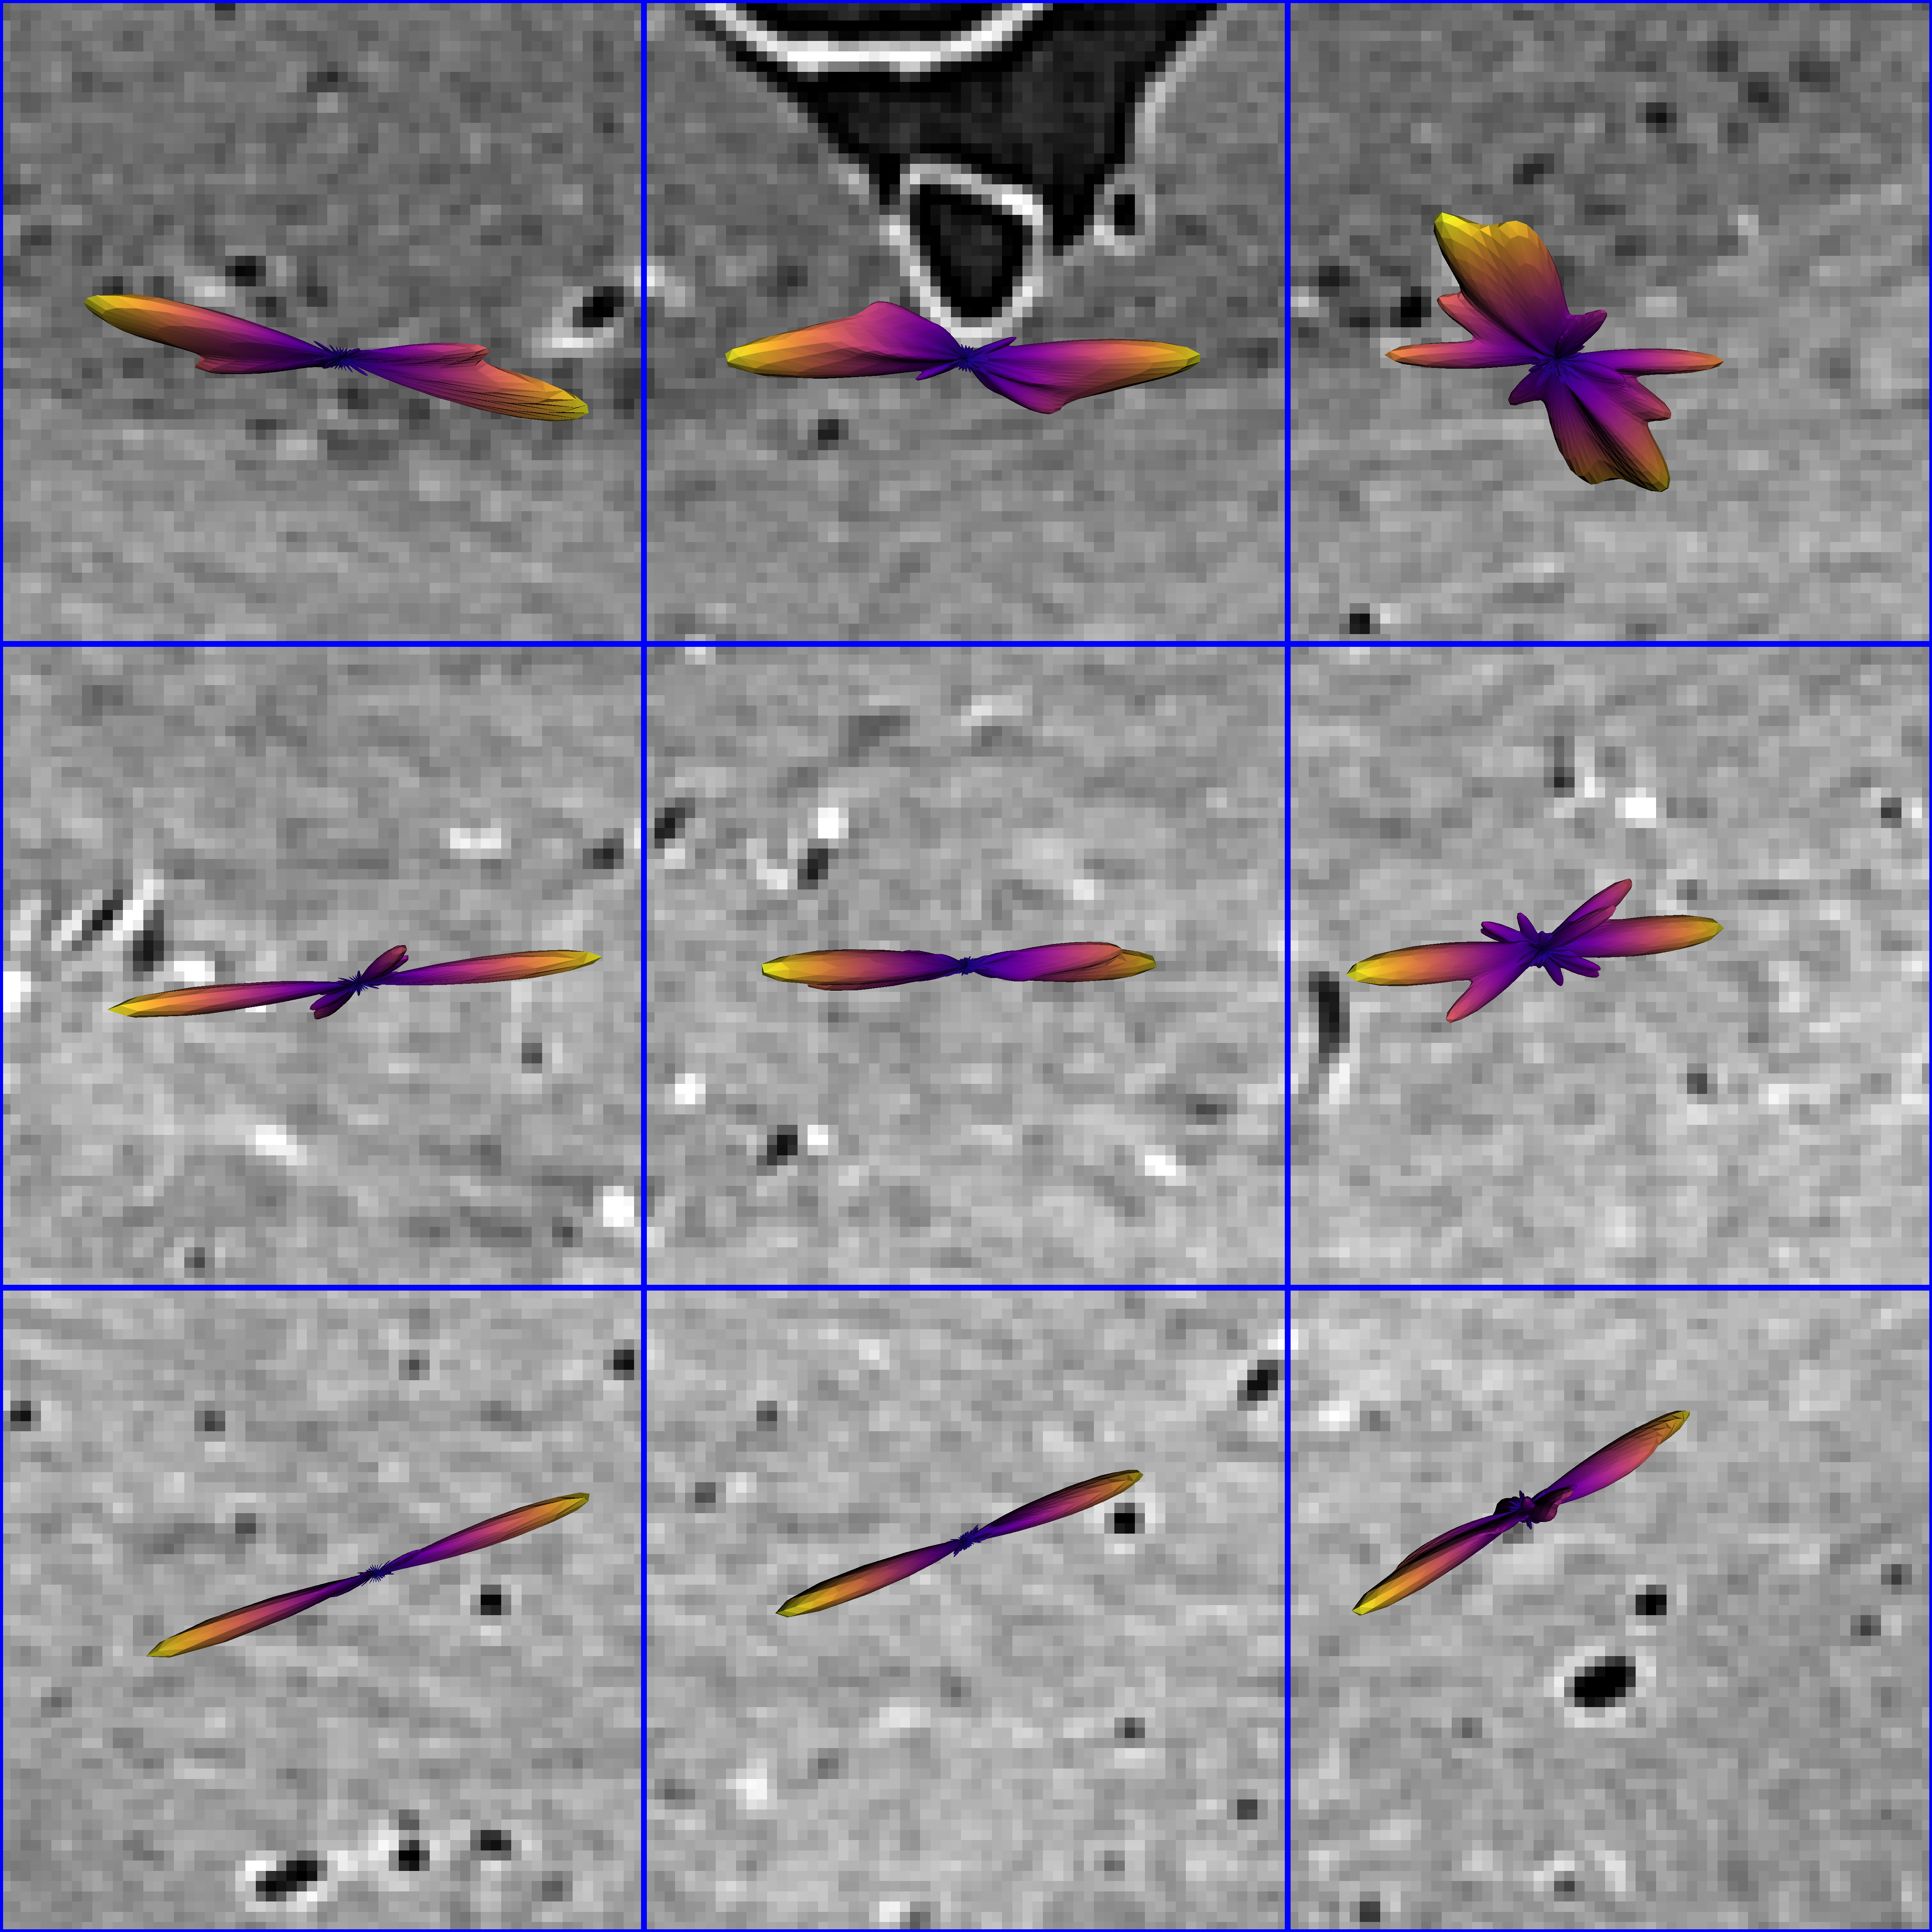
\includegraphics[width=0.4\linewidth]{figs/real_data/CC3} & 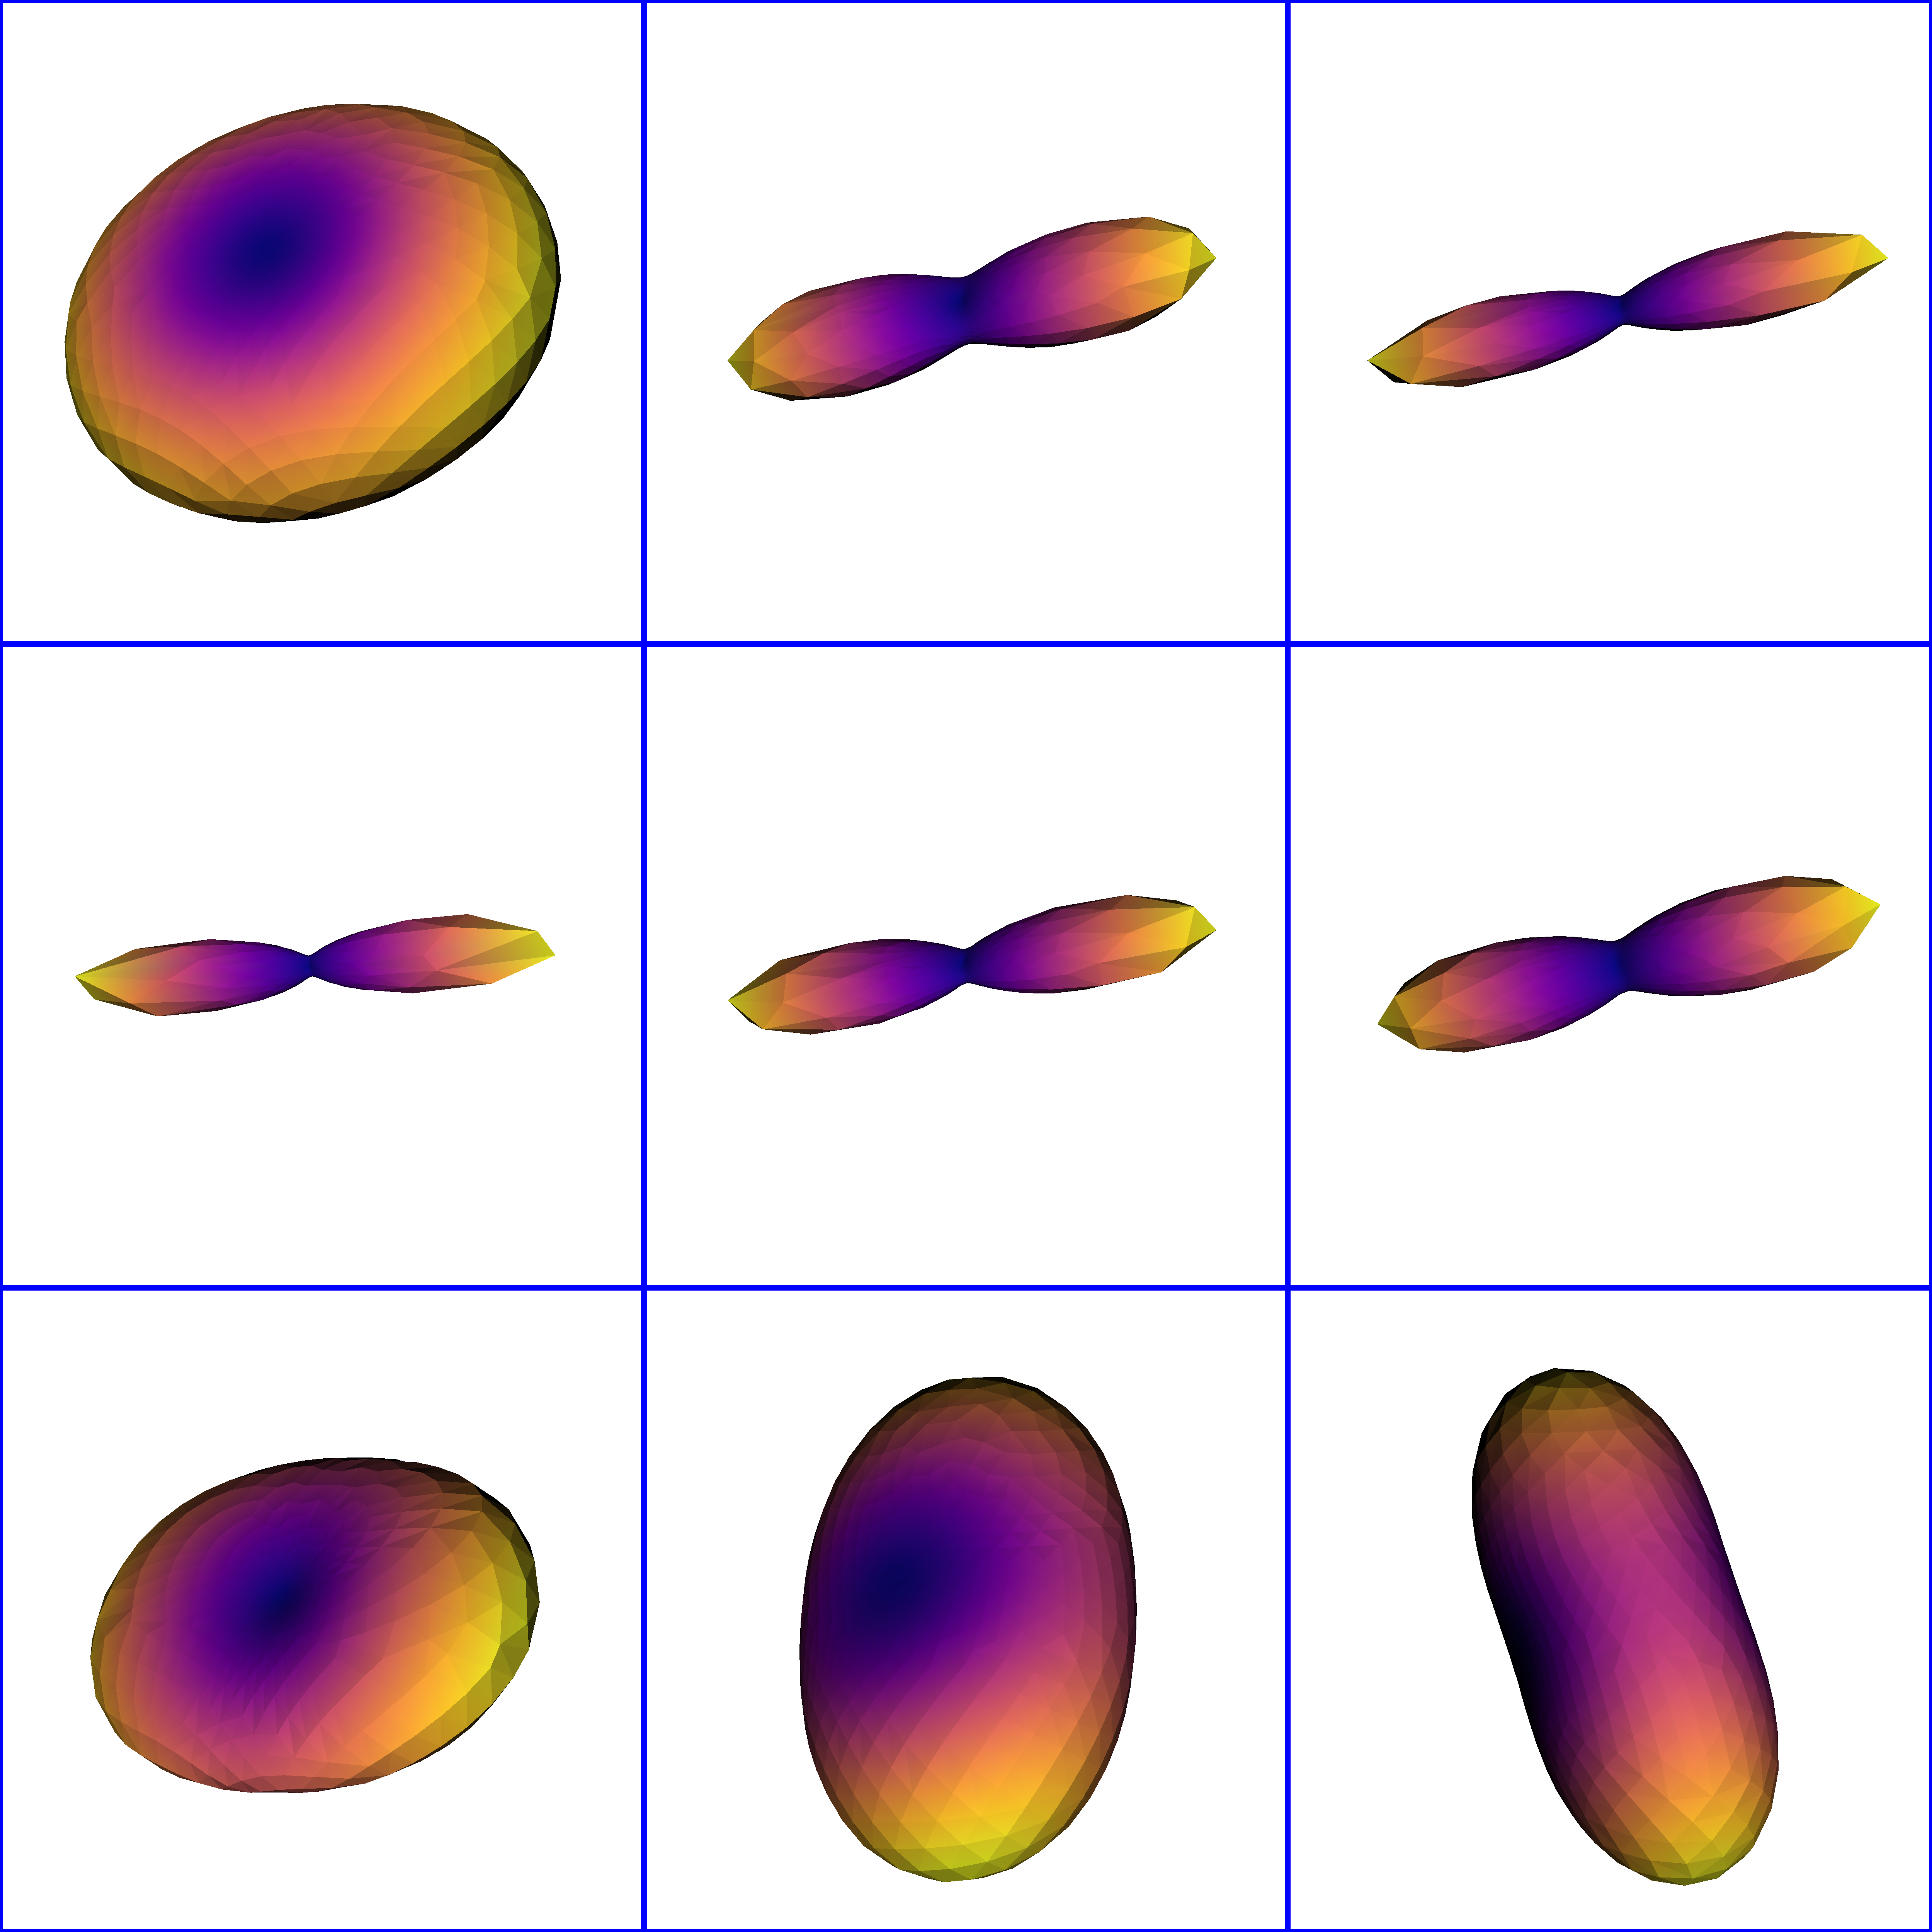
\includegraphics[width=0.4\linewidth]{figs/real_data/CC3_DTI}\\
        $\upmu$CT FODs & DTI FODs
      \end{tabular}
    \end{center}

    \columnbreak
    
    
  \end{multicols}

  \vspace{0.5em}

  \begin{center}
  \begin{tabular}{l}
    \textbf{Figure 1.} (Top) Two representative $\upmu$CT slices with highlighted 450
    $\upmu$m$^3$ ROI containing myelinated nerve fibers. \\
    (Bottom)~$\upmu$CT~FODs are calculated within 150 $\upmu$m$^3$ ROI -- the size of a single dMRI
    voxel -- using spherical harmonic \\
    coefficients up to $L_{max}=20$. For qualitative comparison, ROI from similar locations in the dMRI data were chosen \\
    and FODs were reconstructed using the diffusion tensor model (DTI).\\
  \end{tabular}
  \end{center}
}
\setlength{\columnsep}{1.5em}

% ----------------------------------------------------------------------------------------
%	Discussion
%----------------------------------------------------------------------------------------

  \headerbox{Discussion}{name=discussion, column=3, row=0}{
    \vspace{0.5em}

    This work introduces a ground truth dataset with natively isotropic
    resolution that will allow for validation of dMRI FODs over the whole brain,
    with no need for physical sectioning.\newline

    Qualitatively, the peaks identified in the $\upmu$CT FODs align well with
    the visible orientations of the nerve fibers in the intensity data. As a
    preliminary visual comparison, there is also good alignment with the DTI
    FODs over some voxels. Efforts are ongoing to perform the non-linear,
    multi-modality registration of the two datasets needed to account for
    physical warping of the sample during preparation for $\upmu$CT
    imaging.\newline

    Once the $\upmu$CT and dMRI data are registered, FODs will be reconstructed from
    the dMRI data using a number of available algorithms. Quantitative
    comparisons to the $\upmu$CT FODs across the whole brain will provide a wealth
    of information regarding the ability of these algorithms to represent
    microstructural regions of varying complexity
    \vspace{0.5em}
  }

%----------------------------------------------------------------------------------------
%	Future Work
%----------------------------------------------------------------------------------------

  \headerbox{Future Work}{name=future, column=3, below=discussion}{
    \vspace{0.5em}
    New developments in the $\upmu$CT acquisition process will allow sub-micron
    resolution, and the potential to resolve individual myelinated axons. Direct
    segmentation of white matter tracts across the whole brain will provide the
    means for large-scale validation studies in dMRI tractography.\newline

    The sample staining procedure is identical for $\upmu$CT and serial electron
    microscopy. This will allow for follow up imaging of partial regions of
    the same brain tissue with synapse-level resolution, resulting in \textbf{a pipeline of
    complementary imaging techniques with resolution spanning six orders of
    magnitude.}

    \begin{center}
      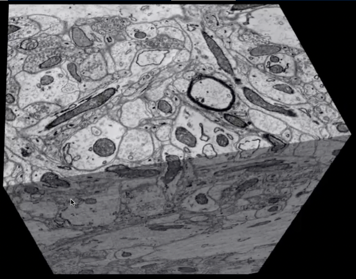
\includegraphics[width=0.37\linewidth]{figs/grant_EM_stack}\\[6pt]
      \begin{tabular}{l}
        \textbf{Figure 2:} 3D serial EM stack of neural tissue,
        with \\resolution of 3 nm $\times$ 3 nm $\times$ 30 nm over a FOV of 40 $\upmu$m$^3$.
        \end{tabular}
    \end{center}
  }

  
%----------------------------------------------------------------------------------------
%	References
%----------------------------------------------------------------------------------------

\headerbox{References}{name=references,column=3, above=bottom}{ 
  \renewcommand{\section}[2]{\vskip0.05em} % Get rid of the default "References" section title
  % \nocite{*} % Insert publications even if they are not cited in the poster
  \scriptsize{ % Reduce the font size in this block
    \bibliographystyle{ieeetr}
    \bibliography{gordonposterbib} % Use sample.bib as the bibliography file
  }
}
\end{poster}
\end{document}